 \documentclass[12pt,twoside]{article}

\newcommand{\reporttitle}{Machine Learning}
\newcommand{\reportauthor}{Dimitrogiannis Kontogouris, Michael Tarasiou}
\newcommand{\reporttype}{CBC: Neural Networks}
\newcommand{\cid}{00650270, 00661239}
\usepackage{amsmath}
\usepackage{listings}
\usepackage{lscape}
\usepackage{float}

% include files that load packages and define macros
%%%%%%%%%%%%%%%%%%%%%%%%%%%%%%%%%%%%%%%%%
% University Assignment Title Page 
% LaTeX Template
% Version 1.0 (27/12/12)
%
% This template has been downloaded from:
% http://www.LaTeXTemplates.com
%
% Original author:
% WikiBooks (http://en.wikibooks.org/wiki/LaTeX/Title_Creation)
%
% License:
% CC BY-NC-SA 3.0 (http://creativecommons.org/licenses/by-nc-sa/3.0/)
% 
% Instructions for using this template:
% This title page is capable of being compiled as is. This is not useful for 
% including it in another document. To do this, you have two options: 
%
% 1) Copy/paste everything between \begin{document} and \end{document} 
% starting at \begin{titlepage} and paste this into another LaTeX file where you 
% want your title page.
% OR
% 2) Remove everything outside the \begin{titlepage} and \end{titlepage} and 
% move this file to the same directory as the LaTeX file you wish to add it to. 
% Then add \input{./title_page_1.tex} to your LaTeX file where you want your
% title page.
%
%----------------------------------------------------------------------------------------
%	PACKAGES AND OTHER DOCUMENT CONFIGURATIONS
%----------------------------------------------------------------------------------------
\usepackage{ifxetex}
\usepackage{textpos}
\usepackage{natbib}
\usepackage{kpfonts}
\usepackage[a4paper,hmargin=2.8cm,vmargin=2.0cm,includeheadfoot]{geometry}
\usepackage{ifxetex}
\usepackage{stackengine}
\usepackage{tabularx,longtable,multirow,subfigure,caption}%hangcaption
\usepackage{fncylab} %formatting of labels
\usepackage{fancyhdr}
\usepackage{color}
\usepackage[tight,ugly]{units}
\usepackage{url}
\usepackage{float}
\usepackage[english]{babel}
\usepackage{amsmath}
\usepackage{graphicx}
\usepackage[colorinlistoftodos]{todonotes}
\usepackage{dsfont}
\usepackage{epstopdf} % automatically replace .eps with .pdf in graphics
\usepackage{natbib}
\usepackage{backref}
\usepackage{array}
\usepackage{latexsym}
\usepackage{etoolbox}

\usepackage{enumerate} % for numbering with [a)] format 



\ifxetex
\usepackage{fontspec}
\setmainfont[Scale=.8]{OpenDyslexic-Regular}
\else
\usepackage[pdftex,pagebackref,hypertexnames=false,colorlinks]{hyperref} % provide links in pdf
\hypersetup{pdftitle={},
  pdfsubject={}, 
  pdfauthor={\reportauthor},
  pdfkeywords={}, 
  pdfstartview=FitH,
  pdfpagemode={UseOutlines},% None, FullScreen, UseOutlines
  bookmarksnumbered=true, bookmarksopen=true, colorlinks,
    citecolor=black,%
    filecolor=black,%
    linkcolor=black,%
    urlcolor=black}
\usepackage[all]{hypcap}
\fi

\usepackage{tcolorbox}

% various theorems
\usepackage{ntheorem}
\theoremstyle{break}
\newtheorem{lemma}{Lemma}
\newtheorem{theorem}{Theorem}
\newtheorem{remark}{Remark}
\newtheorem{definition}{Definition}
\newtheorem{proof}{Proof}

% example-environment
\newenvironment{example}[1][]
{ 
\vspace{4mm}
\noindent\makebox[\linewidth]{\rule{\hsize}{1.5pt}}
\textbf{Example #1}\\
}
{ 
\noindent\newline\makebox[\linewidth]{\rule{\hsize}{1.0pt}}
}



%\renewcommand{\rmdefault}{pplx} % Palatino
% \renewcommand{\rmdefault}{put} % Utopia

\ifxetex
\else
\renewcommand*{\rmdefault}{bch} % Charter
\renewcommand*{\ttdefault}{cmtt} % Computer Modern Typewriter
%\renewcommand*{\rmdefault}{phv} % Helvetica
%\renewcommand*{\rmdefault}{iwona} % Avant Garde
\fi

\setlength{\parindent}{0em}  % indentation of paragraph

\setlength{\headheight}{14.5pt}
\pagestyle{fancy}
\fancyfoot[ER,OL]{\thepage}%Page no. in the left on
                                %odd pages and on right on even pages
\fancyfoot[OC,EC]{\sffamily }
\renewcommand{\headrulewidth}{0.1pt}
\renewcommand{\footrulewidth}{0.1pt}
\captionsetup{margin=10pt,font=small,labelfont=bf}


%--- chapter heading

\def\@makechapterhead#1{%
  \vspace*{10\p@}%
  {\parindent \z@ \raggedright %\sffamily
        %{\Large \MakeUppercase{\@chapapp} \space \thechapter}
        %\\
        %\hrulefill
        %\par\nobreak
        %\vskip 10\p@
    \interlinepenalty\@M
    \Huge \bfseries 
    \thechapter \space\space #1\par\nobreak
    \vskip 30\p@
  }}

%---chapter heading for \chapter*  
\def\@makeschapterhead#1{%
  \vspace*{10\p@}%
  {\parindent \z@ \raggedright
    \sffamily
    \interlinepenalty\@M
    \Huge \bfseries  
    #1\par\nobreak
    \vskip 30\p@
  }}
  



% %%%%%%%%%%%%% boxit
\def\Beginboxit
   {\par
    \vbox\bgroup
	   \hrule
	   \hbox\bgroup
		  \vrule \kern1.2pt %
		  \vbox\bgroup\kern1.2pt
   }

\def\Endboxit{%
			      \kern1.2pt
		       \egroup
		  \kern1.2pt\vrule
		\egroup
	   \hrule
	 \egroup
   }	

\newenvironment{boxit}{\Beginboxit}{\Endboxit}
\newenvironment{boxit*}{\Beginboxit\hbox to\hsize{}}{\Endboxit}



\allowdisplaybreaks

\makeatletter
\newcounter{elimination@steps}
\newcolumntype{R}[1]{>{\raggedleft\arraybackslash$}p{#1}<{$}}
\def\elimination@num@rights{}
\def\elimination@num@variables{}
\def\elimination@col@width{}
\newenvironment{elimination}[4][0]
{
    \setcounter{elimination@steps}{0}
    \def\elimination@num@rights{#1}
    \def\elimination@num@variables{#2}
    \def\elimination@col@width{#3}
    \renewcommand{\arraystretch}{#4}
    \start@align\@ne\st@rredtrue\m@ne
}
{
    \endalign
    \ignorespacesafterend
}
\newcommand{\eliminationstep}[2]
{
    \ifnum\value{elimination@steps}>0\leadsto\quad\fi
    \left[
        \ifnum\elimination@num@rights>0
            \begin{array}
            {@{}*{\elimination@num@variables}{R{\elimination@col@width}}
            |@{}*{\elimination@num@rights}{R{\elimination@col@width}}}
        \else
            \begin{array}
            {@{}*{\elimination@num@variables}{R{\elimination@col@width}}}
        \fi
            #1
        \end{array}
    \right]
    & 
    \begin{array}{l}
        #2
    \end{array}
    &%                                    moved second & here
    \addtocounter{elimination@steps}{1}
}
\makeatother

%% Fast macro for column vectors
\makeatletter  
\def\colvec#1{\expandafter\colvec@i#1,,,,,,,,,\@nil}
\def\colvec@i#1,#2,#3,#4,#5,#6,#7,#8,#9\@nil{% 
  \ifx$#2$ \begin{bmatrix}#1\end{bmatrix} \else
    \ifx$#3$ \begin{bmatrix}#1\\#2\end{bmatrix} \else
      \ifx$#4$ \begin{bmatrix}#1\\#2\\#3\end{bmatrix}\else
        \ifx$#5$ \begin{bmatrix}#1\\#2\\#3\\#4\end{bmatrix}\else
          \ifx$#6$ \begin{bmatrix}#1\\#2\\#3\\#4\\#5\end{bmatrix}\else
            \ifx$#7$ \begin{bmatrix}#1\\#2\\#3\\#4\\#5\\#6\end{bmatrix}\else
              \ifx$#8$ \begin{bmatrix}#1\\#2\\#3\\#4\\#5\\#6\\#7\end{bmatrix}\else
                 \PackageError{Column Vector}{The vector you tried to write is too big, use bmatrix instead}{Try using the bmatrix environment}
              \fi
            \fi
          \fi
        \fi
      \fi
    \fi
  \fi 
}  
\makeatother

\robustify{\colvec}

%%% Local Variables: 
%%% mode: latex
%%% TeX-master: "notes"
%%% End: 
 % various packages needed for maths etc.
% quick way of adding a figure
\newcommand{\fig}[3]{
 \begin{center}
 \scalebox{#3}{\includegraphics[#2]{#1}}
 \end{center}
}

%\newcommand*{\point}[1]{\vec{\mkern0mu#1}}
\newcommand{\ci}[0]{\perp\!\!\!\!\!\perp} % conditional independence
\newcommand{\point}[1]{{#1}} % points 
\renewcommand{\vec}[1]{{\boldsymbol{{#1}}}} % vector
\newcommand{\mat}[1]{{\boldsymbol{{#1}}}} % matrix
\newcommand{\R}[0]{\mathds{R}} % real numbers
\newcommand{\Z}[0]{\mathds{Z}} % integers
\newcommand{\N}[0]{\mathds{N}} % natural numbers
\newcommand{\nat}[0]{\mathds{N}} % natural numbers
\newcommand{\Q}[0]{\mathds{Q}} % rational numbers
\ifxetex
\newcommand{\C}[0]{\mathds{C}} % complex numbers
\else
\newcommand{\C}[0]{\mathds{C}} % complex numbers
\fi
\newcommand{\tr}[0]{\text{tr}} % trace
\renewcommand{\d}[0]{\mathrm{d}} % total derivative
\newcommand{\inv}{^{-1}} % inverse
\newcommand{\id}{\mathrm{id}} % identity mapping
\renewcommand{\dim}{\mathrm{dim}} % dimension
\newcommand{\rank}[0]{\mathrm{rk}} % rank
\newcommand{\determ}[1]{\mathrm{det}(#1)} % determinant
\newcommand{\scp}[2]{\langle #1 , #2 \rangle}
\newcommand{\kernel}[0]{\mathrm{ker}} % kernel/nullspace
\newcommand{\img}[0]{\mathrm{Im}} % image
\newcommand{\idx}[1]{{(#1)}}
\DeclareMathOperator*{\diag}{diag}
\newcommand{\E}{\mathds{E}} % expectation
\newcommand{\var}{\mathds{V}} % variance
\newcommand{\gauss}[2]{\mathcal{N}\big(#1,\,#2\big)} % gaussian distribution N(.,.)
\newcommand{\gaussx}[3]{\mathcal{N}\big(#1\,|\,#2,\,#3\big)} % gaussian distribution N(.|.,.)
\newcommand{\gaussBig}[2]{\mathcal{N}\left(#1,\,#2\right)} % see above, but with brackets that adjust to the height of the arguments
\newcommand{\gaussxBig}[3]{\mathcal{N}\left(#1\,|\,#2,\,#3\right)} % see above, but with brackets that adjust to the height of the arguments
\DeclareMathOperator{\cov}{Cov} % covariance (matrix) 
\ifxetex
\renewcommand{\T}[0]{^\top} % transpose
\else
\newcommand{\T}[0]{^\top}
\fi
% matrix determinant
\newcommand{\matdet}[1]{
\left|
\begin{matrix}
#1
\end{matrix}
\right|
}



%%% various color definitions
\definecolor{darkgreen}{rgb}{0,0.6,0}

\newcommand{\blue}[1]{{\color{blue}#1}}
\newcommand{\red}[1]{{\color{red}#1}}
\newcommand{\green}[1]{{\color{darkgreen}#1}}
\newcommand{\orange}[1]{{\color{orange}#1}}
\newcommand{\magenta}[1]{{\color{magenta}#1}}
\newcommand{\cyan}[1]{{\color{cyan}#1}}


% redefine emph
\renewcommand{\emph}[1]{\blue{\bf{#1}}}

% place a colored box around a character
\gdef\colchar#1#2{%
  \tikz[baseline]{%
  \node[anchor=base,inner sep=2pt,outer sep=0pt,fill = #2!20] {#1};
    }%
}%
 % short-hand notation and macros


%%%%%%%%%%%%%%%%%%%%%%%%%%%%

\begin{document}
% front page
% Last modification: 2016-09-29 (Marc Deisenroth)
\begin{titlepage}

\newcommand{\HRule}{\rule{\linewidth}{0.5mm}} % Defines a new command for the horizontal lines, change thickness here


%----------------------------------------------------------------------------------------
%	LOGO SECTION
%----------------------------------------------------------------------------------------


\includegraphics[width = 4cm]{./figures/imperial}\\[0.5cm] 

\begin{center} % Center remainder of the page

%----------------------------------------------------------------------------------------
%	HEADING SECTIONS
%----------------------------------------------------------------------------------------
\textsc{\LARGE \reporttype}\\[1.5cm] 
\textsc{\Large Imperial College London}\\[0.5cm] 
\textsc{\large Department of Computing}\\[0.5cm] 
%----------------------------------------------------------------------------------------
%	TITLE SECTION
%----------------------------------------------------------------------------------------

\HRule \\[0.4cm]
{ \huge \bfseries \reporttitle}\\ % Title of your document
\HRule \\[1.5cm]
\end{center}
%----------------------------------------------------------------------------------------
%	AUTHOR SECTION
%----------------------------------------------------------------------------------------

%\begin{minipage}{0.4\hsize}
\begin{flushleft} \large
\textit{Author:}\\
\reportauthor~(CID: \cid) % Your name
\end{flushleft}
\vspace{2cm}
\makeatletter
Date: \@date 

\vfill % Fill the rest of the page with whitespace



\makeatother


\end{titlepage}



%%%%%%%%%%%%%%%%%%%%%%%%%%%% Main document


\section{Linear and Relu layers}
All functions discussed below work for any size of input variable or its derivatives. In functions that include linear transormations, to get the dimensionality correct we reshape the input variable $X$ to $NxD$ where $D$ is the unrolled dimensionality of a sample (product of all but the first dimension, the first dimension corresponds to number of samples). The weights of the neural network are matrices of dimensions $DxB$ where $B$ is the dimension of the next layer. Bias terms are $b \in \R^B$ and are broadcasted when added to matrices. 
\subsection{Linear forward pass}

The linear forward function performs a linear transformation to the incoming data matrix $X \in \mathbb{R}^{N \times D}$, transforming it into a matrix $y \in \mathbb{R}^{N \times B}$ where $B$ is the number of neurons in the next layer of the network. Mathematically this is shown below:
\begin{align}
y = XW + b
\end{align}

\subsection{Linear backward pass}

For the backward pass, we are asked to return the derivatives of the loss function with respect to the weights and biases in the layer and the input X.
We have:
\begin{align}
dw = \frac{\partial L}{\partial w} = \frac{\partial L}{\partial y} \times \frac{\partial y}{\partial w}
\end{align}
\begin{align*}
\frac{\partial y}{\partial w} = \frac{\partial (XW + b)}{\partial w} = X
\end{align*}

We know $\frac{\partial L}{\partial y}$ since it is a function input (dout) and thus we can calculate $dw$:
\begin{align}
dw = \frac{\partial L}{\partial w} = \frac{\partial L}{\partial y} \times X = dout \times X
\end{align}
Similarly, the gradient with respect to the biases is:
\begin{align*}
db = \frac{\partial L}{\partial b} = \frac{\partial L}{\partial y} \times \frac{\partial y}{\partial b} = \frac{\partial L}{\partial y} \times 1 = \frac{\partial L}{\partial y} = dout
\end{align*}

Finally, the gradient with respect to the input X:
\begin{align}
dX = \frac{\partial L}{\partial X} = \frac{\partial L}{\partial y} \times \frac{\partial y}{\partial X} = \frac{\partial L}{\partial y} \times W = dout \times W
\end{align}

The dimensions of the gradients are: $dw \in \mathbb{R}^{D \times B}$, $db \in \mathbb{R}^{N \times B}$ and $dX \in \mathbb{R}^{N \times D}$

\subsection{Relu forward pass}

The relu forward pass is simply defined as:
\begin{align}
y = max(0,X)
\end{align}
The output of the relu forward pass is the input X, if X is greater than 0, otherwise it is 0. The dimensions of matrices $y$ and $X$ are the same $N \times D$ for some $N$ and $D$.

\subsection{Relu backward pass}

The relu backward pass is simply 0 if X less than 0, otherwise it is equal to dout.

\section{Dropout}
Dropout is a method to prevent over-fitting in the neural network by dropping or "disabling" neurons in the layers of the network during training. Each neuron has a probability $p$ of being dropped. During testing we do not use dropout. This leads to an inconsistency of the node activations during training and test time. To alleviate this we perform inverted dropout and scale the incoming node activations by a factor of $1/(1-p)$ during train time. At test time we can do a forward pass without dropout or scaling. This method ensures minimal interference with the model during test time. 

\subsection{Dropout forward pass}
To perform the dropout forward pass during training, we create a matrix called $mask$ which is of the same shape as the input X, Each element of $mask$, is the equivalent of a random draw from a Bernoulli distribution, with $p$ probability of being $0$, and $1-p$ of being $1$. The output of the layer is an element-wise multiplication of matrix $mask$ and the input $X$, and thus the result is a matrix equal to X, but with some of its elements changed to 0. During test time, no dropout is performed so we just need to return the input variable.

\subsection{Dropout backward pass}

For the backward pass during the training phase, we perform the same operation as for the forward pass in the opposite direction. We multiply the scaling factor, with the mask (the same as before!) and with the derivatives from the next layers. In the testing phase, the derivatives simply pass through, without a mask. 


\section{Softmax}

The output of the neural network produces a number for each of the classes we have in our classification problem. These numbers can be interpreted as un-normalized probabilities. Using a softmax function, we can normalize them to add up to 1 and thus define a discrete probability distribution over the network outputs. Mathematically the softmax function is defined as:

\begin{align}
\sigma_j (y_i) = \frac{e^{y_i[j]}}{\sum_{k=1}^{D} e^{y_i[k]}}
\end{align}

where, D is the number of classes and $y_i \in \mathbb{R}^D$ is a vector with the outputs of the network for each class (of the $i_{th}$ sample). For numerical stability, we multiply (6) both the numerator and denominator by a constant K s.t $\log K = -D$ which improves stability under overflow and has no effect on results.



\subsection{Gradient of softmax}
For the combination of softmax and the negative log likelihood cost function we use, for a label $l \in \R^{D}$ we have the following:

\begin{align*}
L &= - \sum_j l_j \log \sigma_j
\end{align*}

\begin{align*}
\frac{\partial \sigma_j}{\partial y_j} &= \frac{\exp y_j \exp \sum_k y_k - (\exp y_j)^2}{(\sum_k \exp y_k)^2}= \sigma_j (1 - \sigma_j)\\
\\
\frac{\partial \sigma_j}{\partial y_i} &= \frac{-\exp y_j \exp y_i}{(\sum_k \exp y_k)^2}= -\sigma_j \sigma_i, \quad \forall i \neq j
\end{align*}

\begin{align*}
\frac{\partial L}{\partial y_i} &= -\frac{\partial l_i \sigma_i + \sum_{j \neq i}l_j \log \sigma_j}{\partial y_i}\\
&= - l_i \frac{1}{\sigma_i} (1-\sigma_i) \sigma_i + \sum_{j \neq i} l_j \frac{1}{\sigma_j} \sigma_j \sigma_i \\
&= \sigma_i \sum_j l_j - l_i = \sigma_i - l_i
\end{align*}
\section{Question 4}
Both experiments used default learning rate $n = 0.001$ and learning rate decay $0.95$ applied per epoch.\\
For the overfitting task we selected the top 50 images and labels from CIFAR10 and used just those to fit a model. Since the objective was to fit the training data as good as possible with no consideration of generalization capabilities of our network we selected a network with two hidden layers with 1024 and 512 nodes respectively which allow for very complicated functions to be fit. We did not apply any type of regularization as this would penalize the complexity of the model. The selected model achieves $100\%$ accuracy over the training set at the sixth epoch as can be shown in Fig \ref{fig:overfit} below. Momentum was set at $0.5$.
\\

To get $50\%$ accuracy over the validation set, we selected a network with two hidden layers, 512 and 256 nodes per respective layer. We didn't use dropout, but we did use a $0.2$ $L_2$ regularization multiplier. The model achieved $>50\%$ over the validation set after 4 epochs as can be seen in Fig \ref{fig:cifar_2layer} below. Momentum was set at $0.3$.

\begin{figure}[]
\centering % this centers the figure
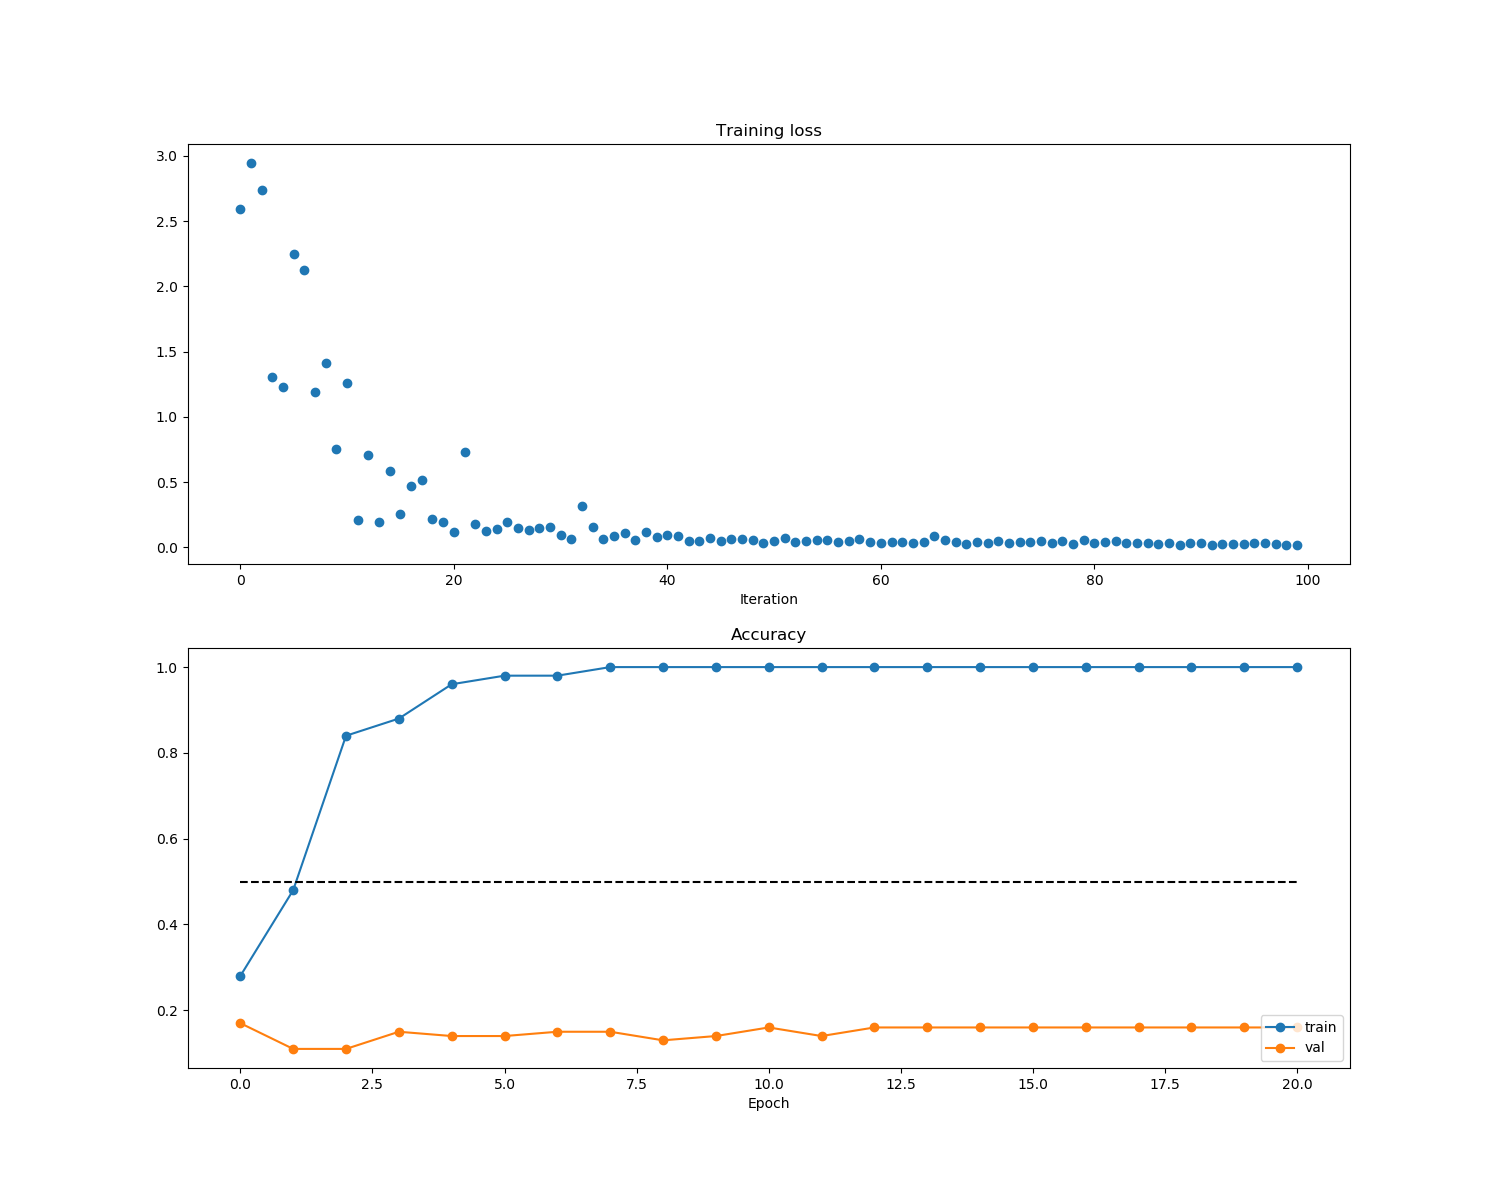
\includegraphics[width = 0.8\hsize]{./figures/overfit.png} % this includes the figure and specifies that it should span 0.7 times the horizontal size of the page
\caption{Network overfitting a subset of CIFAR10 dataset} % caption of the figure
% with a $stepsize$ $0.06$ and starting point $[1, -1]^T$
\label{fig:overfit} % a label. When we refer to this label from the text, the figure number is included automatically
\end{figure}

\begin{figure}[]
\centering % this centers the figure
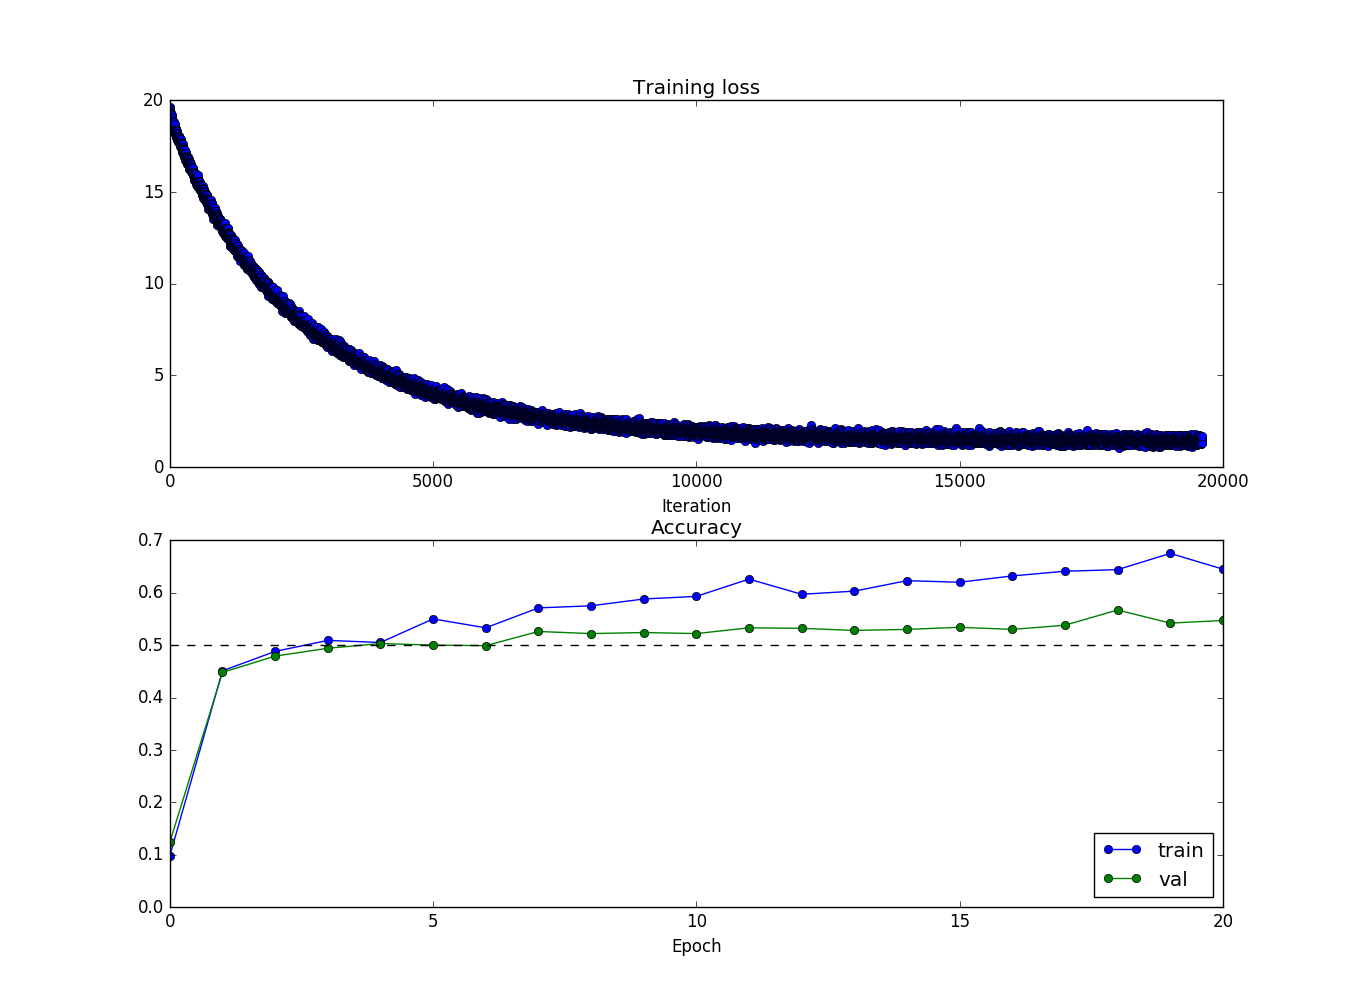
\includegraphics[width = 0.8\hsize]{./figures/cifar_2layer.png} % this includes the figure and specifies that it should span 0.7 times the horizontal size of the page
\caption{Network achieving $>50\%$ validation accuracy in CIFAR10 dataset} % caption of the figure
% with a $stepsize$ $0.06$ and starting point $[1, -1]^T$
\label{fig:cifar_2layer} % a label. When we refer to this label from the text, the figure number is included automatically
\end{figure}

\section{Hyper-parameter Optimization}

For an initial model architecture we have decided to use 2 hidden layers. That choice was motivated by the following. Any single hidden layer feed-forward neural network is proven to be a universal function approximator for a large enough number of hidden units so in theory a single hidden layer network is enough to represent the function we want to find. In practice, a single hidden layer network may require up to an exponential (to the input) number of hidden units to express a function and deep networks can approximate the same function using fewer parameters. Our problem is classifying human emotion which is very likely a complicated function that can benefit from multiple hidden layers. For all things equal simpler is better and less computation and complication are easier to manage. For that reason we decided not to use many hidden layers at the beginning. In addition, a two layer neural network was used in the CIFAR dataset achieving classification scores above 50\%. The CIFAR dataset has a comparable number of input units to FER2013 so using an NN of similar size seems like a good starting point.

In terms of the activation units for the hidden layers, we are using rectified linear units (ReLu). Networks using ReLu allow more efficient back propagation and have been proven to outperform networks with other activation functions. For that reason we will not be experimenting with different activation functions. For the output layer alone we are using a softmax layer which generalizes sigmoid activations to multiple output units and is ideal for the multi class classification problem at hand.

In general we want to reduce the learning rate as time progresses and we are reaching the local minimum. We use the default learning rate decay update schedule, reducing the learning rate by a given factor after each epoch, which satisfies this requirement and is simple enough.


The \textbf{stopping criterion} we choose is early stopping, that is to stop training if the validation set accuracy has not increased over a number of 10 consecutive training epochs.


To optimize the hyper-parameters of the neural network, we used a 2 layer network configuration with \textbf{512 and 256 neurons} in the first and second hidden layer respectively. To train the network, we used \textbf{stochastic gradient descent with momentum 0.9} and a \textbf{batch size of 100}, since it seemed to provide the best compromise between training time and validation performance. Finally, we used \textbf{50 epochs}, but in many cases the training stopped earlier due to the stopping criterion. 
\newline

For the optimization of each parameter, we fix all other parameters, and manually optimize only the variable at hand by repeated cycles of training and assessing the performance of the neural network.
\subsection{Learning rate optimization}

To optimize the learning rate we trained the network with the configuration as described above  using 4 different learning rates and observed the training and validation accuracy. For this optimization, we did not include L2 regularization or dropout. In addition, we did not have any rate decay between epochs.


\begin{table}[!htbp]
\centering
\label{my-label}
\begin{tabular}{|l|c|c|c|}
\hline
\textit{\textbf{LR}} & \multicolumn{1}{l|}{\textit{\textbf{Validation Accuracy (\%)}}} & \multicolumn{1}{l|}{\textit{\textbf{Train Accuracy (\%)}}} & \multicolumn{1}{l|}{\textit{\textbf{Minimum loss achieved}}} \\ \hline
0.0001                          & 40.28                                                           & 51.1                                                       & 1.1770                                                       \\ \hline
0.001                           & 42.09                                                           & 79.1                                                       & 0.4454                                                       \\ \hline
0.01                            & 45.08                                                           & 98.0                                                       & 0.0069                                                       \\ \hline
0.1                             & 26.90                                                           & 27.5                                                       & 1.5881                                                       \\ \hline
\end{tabular}
\caption{Learning rate optimization}
\label{Learning rate optimization}
\end{table}

As it is shown from table \ref{Learning rate optimization}, the best performing model was achieved with a learning rate of $0.01$, with a validation accuracy of 45.08\%.
Figure \ref{lrate0_01} shows the training and validation accuracy vs the number of epochs, as well as the training loss for learning rate 0.01.
Figure \ref{learnin_rate_val_acc} shows the best validation accuracy achieved for different learning rates between $10^{-5}$ and $10^{-1}$. Once again the plot shows that the best choice of learning rate is around $10^{-2}$.

\begin{figure}[!htbp]
\centering % this centers the figure
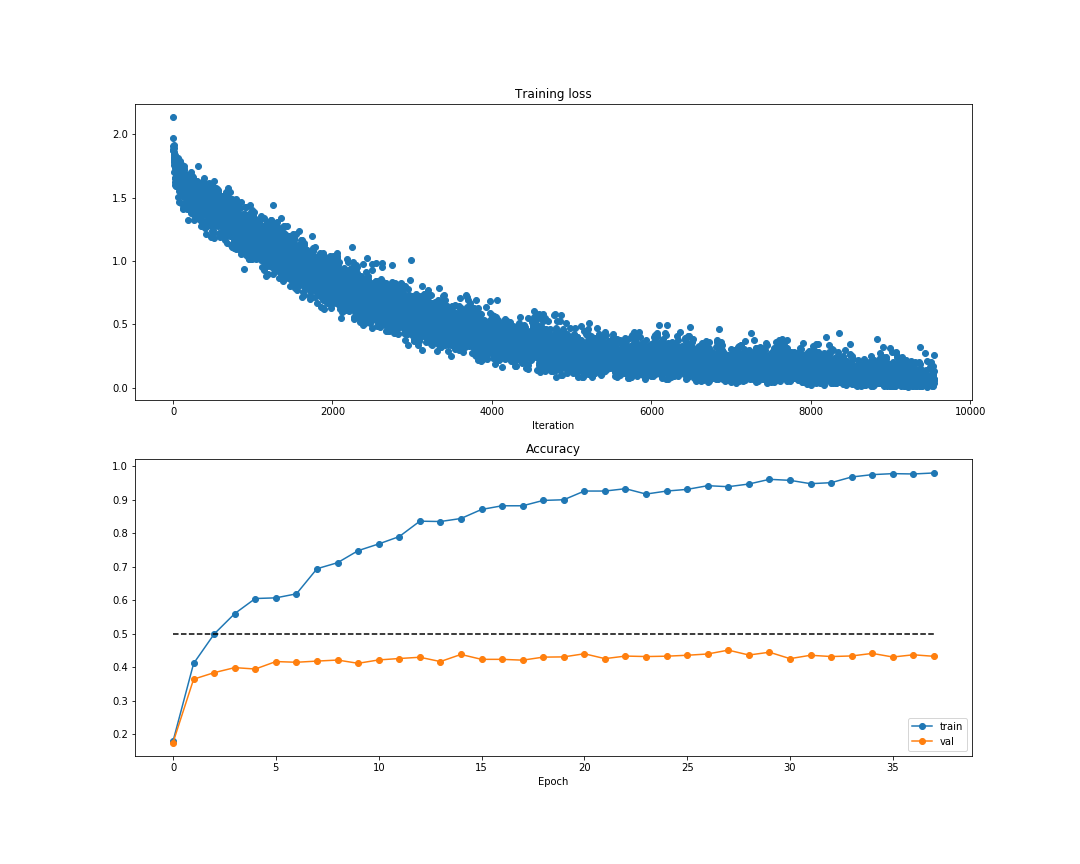
\includegraphics[width = 0.8\hsize]{./figures/l_rate_0_01.png} % this includes the figure and specifies that it should span 0.7 times the horizontal size of the page
\caption{Learning rate: 0.01. \textbf{Top}: Training loss vs number of iterations, \textbf{Bottom}: Training and Validation accuracy vs epochs} % caption of the figure
\label{lrate0_01}
\end{figure}

\begin{figure}[!htbp]
\centering % this centers the figure
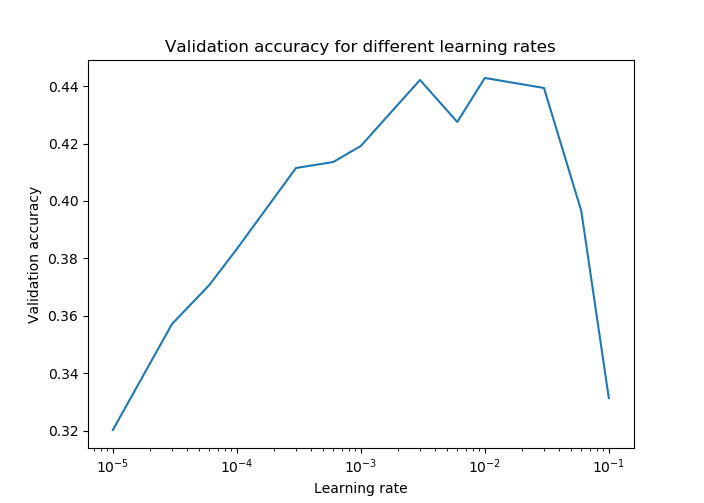
\includegraphics[width = 0.8\hsize]{./figures/learning_rate_val_accuracy.png} % this includes the figure and specifies that it should span 0.7 times the horizontal size of the page
\caption{Validation accuracy for different learning rates} % caption of the figure
\label{learnin_rate_val_acc}
\end{figure}


\begin{figure}[!htbp]
\centering % this centers the figure
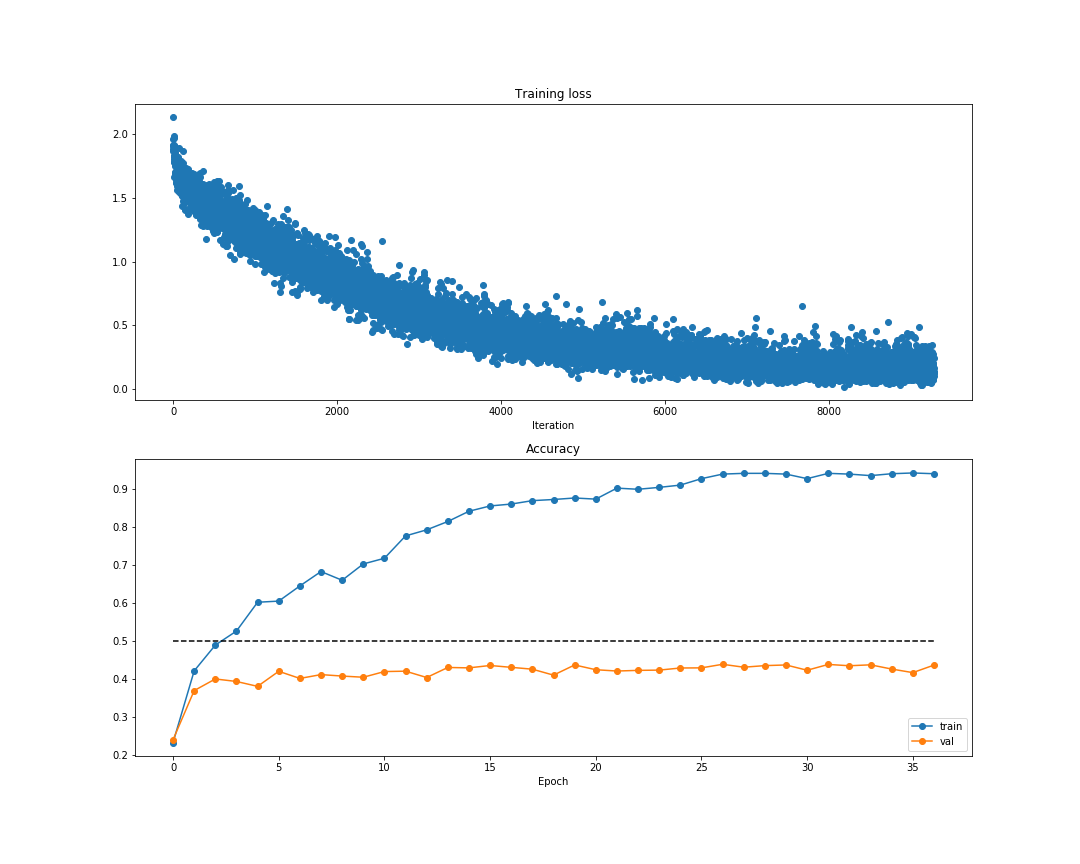
\includegraphics[width = 0.8\hsize]{./figures/drop_0_01.png} % this includes the figure and specifies that it should span 0.7 times the horizontal size of the page
\caption{Dropout: 0.01. \textbf{Top}: Training loss vs number of iterations, \textbf{Bottom}: Training and Validation accuracy vs epochs} % caption of the figure
\label{dropout0_01}
\end{figure}

\subsection{Dropout optimization}

Using the optimized learning rate from the previous section, 0.01, we trained the network once again fixing all parameters except the probability of dropout. We tested four probabilities of dropout 0.01, 0.02, 0.05 and 0.1. 

\begin{table}[!htbp]
\centering
\begin{tabular}{|l|c|c|c|}
\hline
\textit{\textbf{Dropout}} & \multicolumn{1}{l|}{\textit{\textbf{Validation Accuracy (\%)}}} & \multicolumn{1}{l|}{\textit{\textbf{Train Accuracy (\%)}}} & \multicolumn{1}{l|}{\textit{\textbf{Minimum loss achieved}}} \\ \hline
0.01                      & 43.83                                                           & 94.3                                                       & 0.021                                                        \\ \hline
0.02                      & 43.97                                                           & 93.9                                                       & 0.055                                                        \\ \hline
0.05                      & 42.19                                                           & 81.6                                                       & 0.296                                                        \\ \hline
0.1                       & 41.64                                                           & 81.4                                                       & 0.286                                                        \\ \hline
\end{tabular}
\caption{Results for different dropout probabilities}
\label{dropout}
\end{table}

We observe from table \ref{dropout} that a dropout rate of 1-2\% seem to perform the best on the validation data, so dropout overall does not seem to help our network. This can be taken as an indication that the network we are training does not have the capacity to benefit from dropout. Figure \ref{dropout0_01} shows the training and validation accuracy as well as the training loss for dropout rate of 0.01. 

\subsection{L2 regularization vs dropout}

To test L2 regularization, we set dropout to 0 and fix all other parameters once again. The results are shown in table \ref{regularization}.

\begin{table}[!htbp]
\centering
\begin{tabular}{|l|c|c|c|}
\hline
\textit{\textbf{Regularization}} & \multicolumn{1}{l|}{\textit{\textbf{Validation Accuracy (\%)}}} & \multicolumn{1}{l|}{\textit{\textbf{Train Accuracy (\%)}}} & \multicolumn{1}{l|}{\textit{\textbf{Minimum loss achieved}}} \\ \hline
0.001                            & 44.28                                                           & 97.0                                                       & 0.1275                                                       \\ \hline
0.01                             & 45.43                                                           & 97.0                                                       & 0.4844                                                       \\ \hline
0.1                              & 43.87                                                           & 61.9                                                       & 1.1971                                                       \\ \hline
1                                & 35.29                                                           & 35.8                                                       & 1.5851                                                       \\ \hline
\end{tabular}
\caption{Results for different regularization parameters}
\label{regularization}
\end{table}

L2 regularization and dropout serve the same purpose which is to improve the generalisation capacity of the fitted model. It is observable from tables \ref{dropout0_01} and \ref{regularization} that as we increase the dropout parameter or the regularization parameter, training accuracy drops, since the model is not "free" to use the parameters that best fit the training data. We observe the best validation performance with regularization set at 0.01 (45.45\%) while for dropout of 0.02 the best validation performance is 43.97\%. Overall, again we notice that our model is in need of little regularization.

\begin{figure}[!htbp]
\centering % this centers the figure
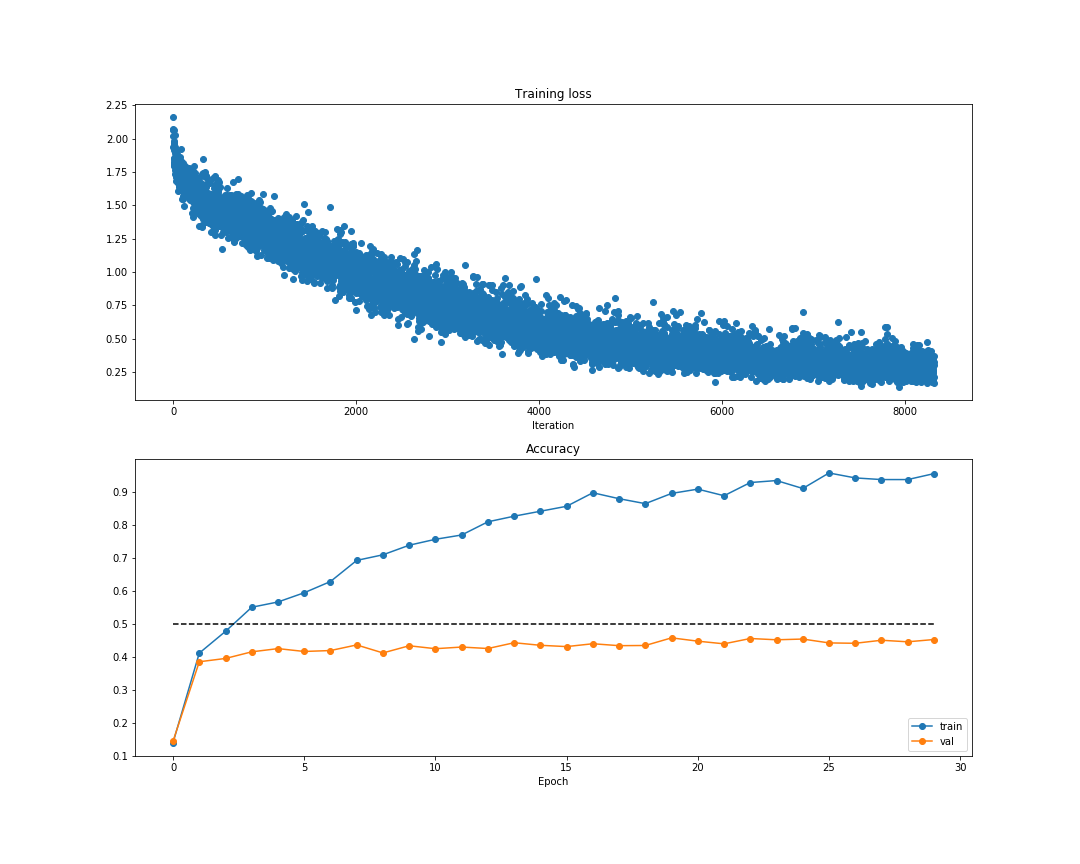
\includegraphics[width = 0.8\hsize]{./figures/reg_0_001.png} % this includes the figure and specifies that it should span 0.7 times the horizontal size of the page
\caption{Regularization: 0.001. \textbf{Top}: Training loss vs number of iterations, \textbf{Bottom}: Training and Validation accuracy vs epochs} % caption of the figure
\label{reg0_001}
\end{figure}

\begin{figure}[!htbp]
\centering % this centers the figure
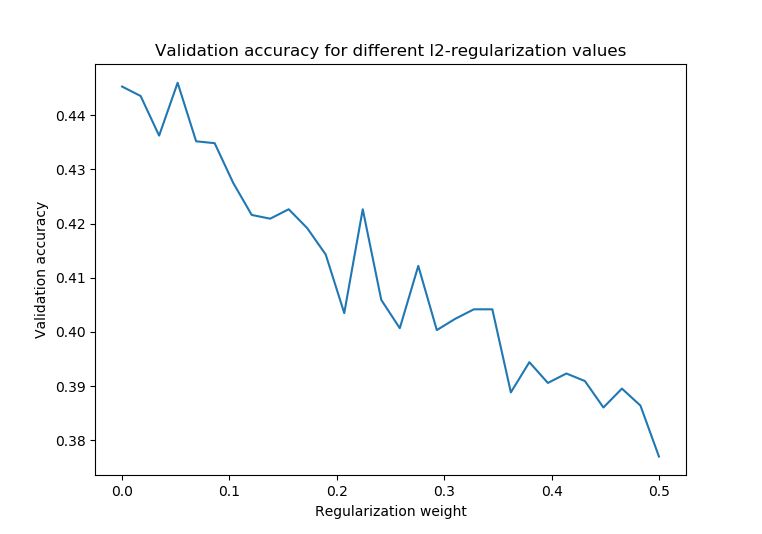
\includegraphics[width = 0.8\hsize]{./figures/regul_val_accuracy.png} % this includes the figure and specifies that it should span 0.7 times the horizontal size of the page
\caption{Validation accuracy for different regularization rates} % caption of the figure
\label{regul_val_acc}
\end{figure}

\newpage
\subsection{Number and size of hidden layers}

Using the optimized parameters, we performed training using different network configurations of 2 or 3 hidden layers,  with different combinations of numbers of nodes per hidden layer. Our general approach was to reduce the number of nodes for deeper layers of the network since our output layer is of only size 7 (7 emotions), while our input layer is 2304 (all the pixels in an image). In addition, we introduce learning rate decay of 95\% (learning rate is reduced by 5\% in each epoch). The results of the optimization are shown below.

\begin{table}[!htbp]
\centering
\begin{tabular}{|l|c|c|c|}
\hline
\textit{\textbf{Architecture}} & \multicolumn{1}{l|}{\textit{\textbf{Validation Accuracy (\%)}}} & \multicolumn{1}{l|}{\textit{\textbf{Train Accuracy (\%)}}} & \multicolumn{1}{l|}{\textit{\textbf{Minimum loss achieved}}} \\ \hline
{[}512, 256{]}                 & 46.93                                                           & 99.9                                                       & 0.458                                                        \\ \hline
{[}256,128{]}                  & 42.47                                                           & 98.9                                                       & 0.3287                                                       \\ \hline
{[}512,512,256{]}              & 44.49                                                           & 97.7                                                       & 0.5950                                                       \\ \hline
{[}512,256,128{]}              & 45.54                                                           & 99.6                                                       & 0.4841                                                       \\ \hline
{[}256,128,64{]}               & 41.67                                                           & 0.7                                                        & 0.8411                                                       \\ \hline
\end{tabular}
\caption{Hidden layers size}
\label{layers}
\end{table}

From table \ref{layers}, we observe that the best validation performance is achieved for the 2 hidden layer NN with 512 and 256 in each of the layers. The validation accuracy is 46.94\%. 


\subsection{Performance of NN on test data}

The NN parameters that are used for this part are the following:
\begin{itemize}
\item 2 hidden layers, 512 and 256 neurons respectively
\item learning rate 0.01 with 0.95 decay
\item dropout probability 0.01
\item regularization 0.01
\item momentum 0.9
\item batch size 100
\item epochs 50
\end{itemize}
Below we analyse the model performance on the test data of FER2013. To get the performance metrics per emotion, we tranformed the predicted classes and the labels to binary values (1 for the emaotion at hand, 0 for all other emotions). The accuracy per emotion is very high, but this does not indicate that the model performs well, since the amount of positive examples in each binary classification (per emotion) is a lot less than the negative examples (all other emotions). Thus, the accuracy is artificially high by predicting the negative examples correctly. The precision, recall and f1 score are better indicators of the performance of the model for each individual emotion. Emotions 5, 3 and 1 exhibit the best performance. The classification rate for all emotions is 46.17\%. The same picture is presented in the confusion matrix shown in Table\ref{confusion}, which shows the actual class (column) given a predicted class (row).


\begin{table}[!htbp]
\centering
\begin{tabular}{|l|c|c|c|c|}
\hline
\textbf{Emotion} & \multicolumn{1}{l|}{\textbf{Accuracy (\%)}} & \multicolumn{1}{l|}{\textbf{Precision (\%)}} & \multicolumn{1}{l|}{\textbf{Recall (\%)}} & \multicolumn{1}{l|}{\textit{\textbf{F1 (\%)}}} \\ \hline
0                & 82.25                                       & 33.0                                         & 35.33                                     & 34.12                                          \\ \hline
1                & 98.55                                       & 54.76                                        & 41.07                                     & 46.94                                          \\ \hline
2                & 82.17                                       & 34.87                                        & 33.47                                     & 34.16                                          \\ \hline
3                & 80.33                                       & 59.89                                        & 63.91                                     & 61.84                                          \\ \hline
4                & 78.54                                       & 39.38                                        & 33.23                                     & 36.05                                          \\ \hline
5                & 91.53                                       & 63.70                                        & 62.17                                     & 62.93                                          \\ \hline
6                & 78.96                                       & 38.78                                        & 42.17                                     & 40.41                                          \\ \hline
\end{tabular}
\caption{Performance of network for each emotion}
\label{performance}
\end{table}

\begin{table}[!htbp]
\centering
\begin{tabular}{|l|c|c|c|c|c|c|c|}
\hline
                     & \multicolumn{1}{l|}{\textit{\textbf{P0}}} & \multicolumn{1}{l|}{\textit{\textbf{P1}}} & \multicolumn{1}{l|}{\textit{\textbf{P2}}} & \multicolumn{1}{l|}{\textit{\textbf{P3}}} & \multicolumn{1}{l|}{\textit{\textbf{P4}}} & \multicolumn{1}{l|}{\textit{\textbf{P5}}} & \multicolumn{1}{l|}{\textit{\textbf{P6}}} \\ \hline
\textit{\textbf{A0}} & 165                                       & 1                                         & 61                                        & 86                                        & 81                                        & 17                                        & 56                                        \\ \hline
\textit{\textbf{A1}} & 8                                         & 23                                        & 4                                         & 6                                         & 8                                         & 1                                         & 6                                         \\ \hline
\textit{\textbf{A2}} & 70                                        & 5                                         & 166                                       & 59                                        & 71                                        & 41                                        & 84                                        \\ \hline
\textit{\textbf{A3}} & 70                                        & 5                                         & 46                                        & 572                                       & 69                                        & 27                                        & 106                                       \\ \hline
\textit{\textbf{A4}} & 86                                        & 5                                         & 90                                        & 106                                       & 217                                       & 30                                        & 119                                       \\ \hline
\textit{\textbf{A5}} & 32                                        & 0                                         & 43                                        & 30                                        & 19                                        & 258                                       & 33                                        \\ \hline
\textit{\textbf{A6}} & 69                                        & 3                                         & 66                                        & 96                                        & 86                                        & 31                                        & 256                                       \\ \hline
\end{tabular}
\caption{Confusion matrix of the test data}
\label{confusion}
\end{table}


\section{Question 6}
For this task we used Tensorflow. The CNN model we submit consists of 4 blocks of convolutional layers (3x3 kernels) followed by max pooling, which are then followed by 2 fully connected layers. We used small 3x3 filters inspired by the VGG architecture that has performed very well in recent years. The stride and padding are selected so that the convolution layer does not modify the size of the features. After each pooling layer we reduce the width and height of the features by a half and double the number of features, effectively halving the total size of the features. We selected a deep convolutional architecture that allows for relatively small size of fully connected layers at the end. The architecture is described in greater detail below:  

\begin{itemize}
\item input layer of dimensions Nx48x48x1 (batch size x image width x image height x number of channels)
\item 2 convolutional layers with 32x3x3x1 filters (number of filters x kernel width x kernel height x number of channels) at stride 1 and 1 zero padding at all dimensions, followed by ReLu activation.  Max pool layer of size 2x2 (width x height) at stride 2 that performs dimensionality reduction. After this step each feature's dimensions are halved leading to a tensor of dimensions Nx24x24x32 (batch size x image width x image height x number of features)
\item 3 convolutional layers with 64x3x3x1 filters at stride 1 and 1 zero padding at all dimensions, followed by ReLu activation. Max pool layer of size 2x2 (width x height) at stride 2. After this step each feature's dimensions are Nx12x12x64 
\item 3 convolutional layers with 128x3x3x1 filters at stride 1 and 1 zero padding at all dimensions, followed by ReLu activation. Max pool layer of size 2x2 (width x height) at stride 2. After this step each feature's dimensions are Nx6x6x128 
\item 3 convolutional layers with 256x3x3x1 filters at stride 1 and 1 zero padding at all dimensions, followed by ReLu activation. Max pool layer of size 2x2 (width x height) at stride 2. After this step each feature's dimensions are Nx3x3x256. This  layer is reshaped to a vector of dimension 2034 and dropout with probability of keeping a node 0.6 (dropout 0.4) is applied
\item fully connected layer with 512 nodes and dropout 0.4
\item fully connected layer with 128 nodes and dropout 0.4
\item output layer of dimension 7 equal to the number of classes
\end{itemize}

Taking advantage of the Tensorflow implementations, we used the Adam optimizer with a learning rate of $0.005$ and default parameters $beta1=0.9$ $beta2=0.999$. Adam was presented in [4] and is a first-order gradient-based optimization that includes adaptive momentum and learning rates. \\


We experimented with using residual networks (ResNet) presented in [1], [2], specifically the 101-layer bottleneck network. Residual networks are one of the most significant advances in terms of convolutional neural network architecture over the last decade. They use what the authors call skip connections between layers that pass identity mappings between the layers they connect. As a result the convolutional layers between skip connections have to model the residual function which is performed more effectively by the network. This architecture option results in more efficient backpropagation and the capacity to train far deeper models that was though achievable before. Our residual networks performed better however due to size limitations we were not able to submit a trained model.\\

The training and validation accuracy with respect to the number of epochs can be seen in Fig.\ref{cnn01} below. Using the Test data to assess performance we get the confusion matrix shown in Table \ref{confusion02} and the precision, recall and F1 scores as shown in Table \ref{confusion02}. Comparing the performancewe can see that the CNN clearly outperforms our best FCN. However that cannot be said regarding all emotions and all performance metrics. For example in the case of emotion A1 (Disgust) the FCN has a higher recall and seems to work equally well when looking at the confusion matrix. Overall, the FER2013 dataset can be difficult to interpret (the human accuracy is about $65\%$ according to [5]) mainly because emotions are rarely present in isolation (human expressions show a mix of emotional states). As such emotion recognition is a complicated task and models are expected to meet a lot of difficulties in fitting it.

\begin{figure}[!htbp]
\centering % this centers the figure
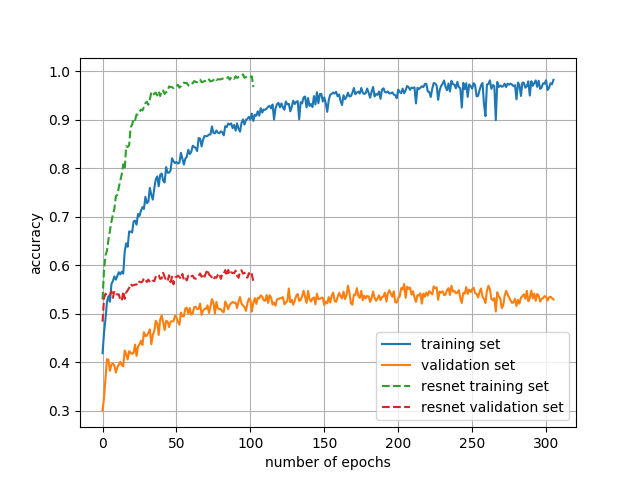
\includegraphics[width = 0.8\hsize]{./figures/cnn_training.png} % this includes the figure and specifies that it should span 0.7 times the horizontal size of the page
\caption{Training and Validation accuracy vs number of epochs} % caption of the figure
\label{cnn01}
\end{figure}

\begin{table}[!htbp]
\centering
\begin{tabular}{|l|c|c|c|c|c|c|c|}
\hline
& \multicolumn{1}{l|}{\textit{\textbf{P0}}} & \multicolumn{1}{l|}{\textit{\textbf{P1}}} & \multicolumn{1}{l|}{\textit{\textbf{P2}}} & \multicolumn{1}{l|}{\textit{\textbf{P3}}} & \multicolumn{1}{l|}{\textit{\textbf{P4}}} & \multicolumn{1}{l|}{\textit{\textbf{P5}}} & \multicolumn{1}{l|}{\textit{\textbf{P6}}} \\ \hline
\textit{\textbf{A0}} & 230&   0&  54&  31&  69&  14&  68 \\ \hline
\textit{\textbf{A1}} &  19&  20&   5&   3&   6&   0&   3 \\ \hline
\textit{\textbf{A2}} & 72&   1& 159&  42&  95&  33&  94 \\ \hline
\textit{\textbf{A3}} & 34&   0&  21& 720&  32&  21&  67 \\ \hline
\textit{\textbf{A4}} & 105&   0&  59&  64& 271&   9& 145 \\ \hline
\textit{\textbf{A5}} & 24&   0&  33&  24&  19& 291&  24  \\ \hline
\textit{\textbf{A6}} & 67&   0&  45&  72& 110&   5& 308 \\ \hline
\end{tabular}
\caption{Confusion matrix of the test data on the trained CNN}
\label{confusion02}
\end{table}


\begin{table}[!htbp]
\centering
\begin{tabular}{|l|c|c|c|c|}
\hline
\textbf{Emotion} & \multicolumn{1}{l|}{\textbf{Accuracy (\%)}} & \multicolumn{1}{l|}{\textbf{Precision (\%)}} & \multicolumn{1}{l|}{\textbf{Recall (\%)}} & \multicolumn{1}{l|}{\textit{\textbf{F1 (\%)}}} \\ \hline
0 & 84.48&  0.42&  0.49&  0.45\\ \hline
1 & 98.97&  0.95&  0.36&  0.52\\ \hline
2 & 84.56&  0.42&  0.32&  0.36\\ \hline
3 & 88.55&  0.75&  0.8 &  0.78\\ \hline
4 & 80.13&  0.45&  0.42&  0.43\\ \hline
5 & 94.26&  0.78&  0.7 &  0.74\\ \hline
6 & 80.49&  0.43&  0.51&  0.47\\ \hline
\end{tabular}
\caption{Performance of CNN per emotion}
\label{performance02}
\end{table}


\section{Additional questions}

\subsection{A1}
We could not claim one to be a better algorithm than the other in general for the following reasons stemming from the fact that the two methods are very different qualitatively:
\begin{itemize}
\item neural networks can be seen as black box function approximators while trees are highly interpretable. In cases where interpretability is crucial we could not use neural networks
\item fitting and doing inference with the two models scales differently depending on the software and hardware architecture used. The computing architecture of today might allow one model to be run more efficiently and outperform the other but that will not necessarily hold for future architectures
\end{itemize}
Finally, the no free lunch theorem for machine learning of [3] states that no apriori distinctions can be made between any two learning algorithms. That is to say that while the inductive principle used by one model might allow it to overperform another at a given problem, when examined under the scope of all possible problems, any two learning algorithms are equivalent.


\subsection{A2}

For the classification trees, adding more classes would require retraining the whole model as the input space for the new classes has to be taken from space previously occupied by other classes. Other than that, the tree algorithm can be applied without changes.\\

For the case of neural networks a step we would definitely need to take is to add another node at the output layer of the network allowing the classification of $n+1$ classes where the previous network was capable of classifying $n$ classes. We will need to initialize the weights and bias connecting the new node with the last hidden layer and we will need to train at least the last layer of the network. Most possibly we will need to retrain the other layers but the previously trained network will provide a good initialization, so it is likely to converge faster than by starting from scratch.

\section{Instructions for executing}
All code was written in Python3. All scripts were tested and run in the DOC Lab environment. To run the submitted scripts open a terminal window in the project directory and follow the instructions below.\\

To run the scripts $test.py$ and $test\_deep.py$ which are used to predict using the best FCN and CNN respectively, use the $src$ as the home directory and complete the user input section at each script. The parameters to complete are $img\_folder$ (the path to the test data) and $srcdir$, the global path to the $src$ directory. Both scripts load the models which are located in subdirectories of the $src$ directory and use the model to make predictions. The predictions are assigned to a variable $preds$ which the user can save to disk or pas it further down the pipeline.The best CNN is named $conv03$ and is saved in subdirectory $src/conv03\_logs$. The best FCN is named $pickle.net$ and is saved in subdirectory $src/pickles$.\\

For the CNN to run tensorflow must be installed.


\section{References}

\begin{verbatim}
[1] Kaiming He, Xiangyu Zhang, Shaoqing Ren, Jian Sun
    Deep Residual Learning for Image Recognition. arXiv:1512.03385

[2] Kaiming He, Xiangyu Zhang, Shaoqing Ren, Jian Sun
    Identity Mappings in Deep Residual Networks. arXiv: 1603.05027
    
[3] Wolpert, David (1996), "The Lack of A Priori Distinctions between 
Learning Algorithms", Neural Computation, pp. 1341-1390

[4] Diederik P. Kingma, Jimmy Ba, " Adam: A Method for Stochastic 
Optimization", arXiv:1412.6980

[5] Goodfeloow et al. "Challenges in Representation Learning: A report 
on three machine learning contests", arXiv:1307.0414
\end{verbatim}




\end{document}
%%% Local Variables: 
%%% mode: latex
%%% TeX-master: t
%%% End: 
